\vspace{1em}
La implementación comentada del algoritmo de Kruskal parece eficiente cuando se trata de grafos ralos pero resulta menos que satisfactoria cuando se trata de estructuras más densas. En particular en este problema, se están ordenando O(n^2) aristas a pesar de que solo se observan n-1 de ellas como máximo.

Afortunadamente contamos con la siguiente especificación: https://fedelebron.com/a-dense-version-of-kruskals-algorithm, que detalla cómo esbozar un algoritmo no sólo más eficiente sino que asintóticamente superior, con complejidad temporal de O(n^2) en vez de O(n^2logn)

Para revisar de manera empírica la diferencia en eficiencia de estas dos implementaciones, procedimos a implementarlas en $C++$ y realizamos una serie de evaluaciones respecto al tiempo de ejecución en función del tamaño de la entrada, para muestras aleatorias de tamaño $n = 5000*k$ para cada $k$ natural en el rango $1 \leq k \leq 10$. Realizamos cada evaluación diez veces para reducir la variación de los resultados y tomamos el promedio aritmético.

Como demás parámetros elegimos w = n/4, r = 1, w = v = 5. Nótese que los valores de cada coordenada (x,y) no afectan el tiempo de ejecución de ninguno de los algoritmos, por lo que simplemente elegimos (i, i+1) con $0 \leq i \leq k*5000$

El siguiente gráfico expone los resultados.

\begin{figure}[!htbp]
    \includegraphics[scale=0.5, clip]{./files/src/.media/comparacion_asintótica.png}
    \caption{Tiempo de ejecución del \textit{cálculo de costos} en función del tamaño de entrada $n$ para el algoritmo \textit{cuadrático} y el \textit{supercuadrático}}
\end{figure}

Se ve que hay una clara diferencia de velocidad a favor del algoritmo cuadrático, incluso en las entradas más pequeñas. Podemos concluir entonces que resulta más eficiente para este problema

\subsection{optimizaciones DSU}

También se nos pide observar si hay diferencia de tiempos al utilizar la estructura de \textit{disjointed set} sin alguna de sus optimizaciones. En este caso obviaremos ambas, \textit{union by rank} y \textit{path compression}. 

Para esto realizamos un algoritmo idéntico al de la práctica pero con funciones diferentes de DSU. A la hora de unir dos sets, recorremos uno, elemento por elemento, y lo agregamos al otro. De acuerdo con el libro de cormen, como hacemos n-w operaciones de make, 2(n-w) find-set y (n-w) uniones, en total tendrá todo una complejidad de O(n + nlogn). Si bien esto no modifica la complejidad total del algoritmo, ciertamente resulta posible que afecte su tiempo de ejecución.

En forma análoga a la experimentación con el algoritmo cuadrático, hacemos una prueba empírica con estos dos algoritmos. El siguiente gráfico mustra los resultados:

\begin{figure}[!htbp]
    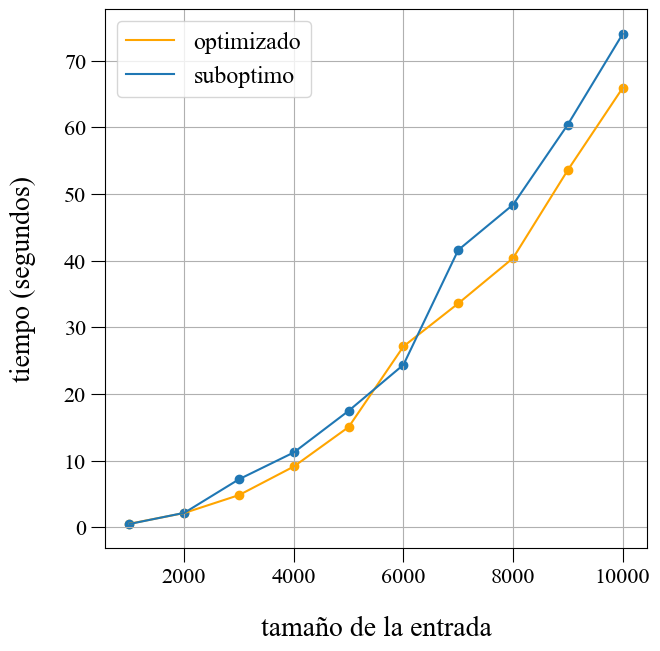
\includegraphics[scale=0.5, clip]{./files/src/.media/comparacion_DSU.png}
    \caption{Tiempo de ejecución del \textit{cálculo de costos} en función del tamaño de entrada $n$ para el algoritmo \textit{optimizado} y el \textit{subóptimo}}
\end{figure}

En las entradas más grandes se ve una diferencia mayor, pero no parece resultar significativa.